\subsection{Path Finding}
In the area of path finding we encounter a few problems due to the desired game mechanics. These problems and their solutions will be discussed in this chapter.

\subsubsection{Navigational Reference \& Exact Positions}
Simply having a map with float co-ordinates makes path finding very difficult due to the endless possibility space. To work with this we put a grid over the map, such that the integer part of a float co-ordinate indexes a cell. This allows us to use graph-based algorithms. Once a unit is in the desired cell, the accuracy of the float number can then fine tune its position.

\subsubsection{Eight-Directional Path Finding on a Grid}
\begin{wrapfigure}{r}{0.30\textwidth}
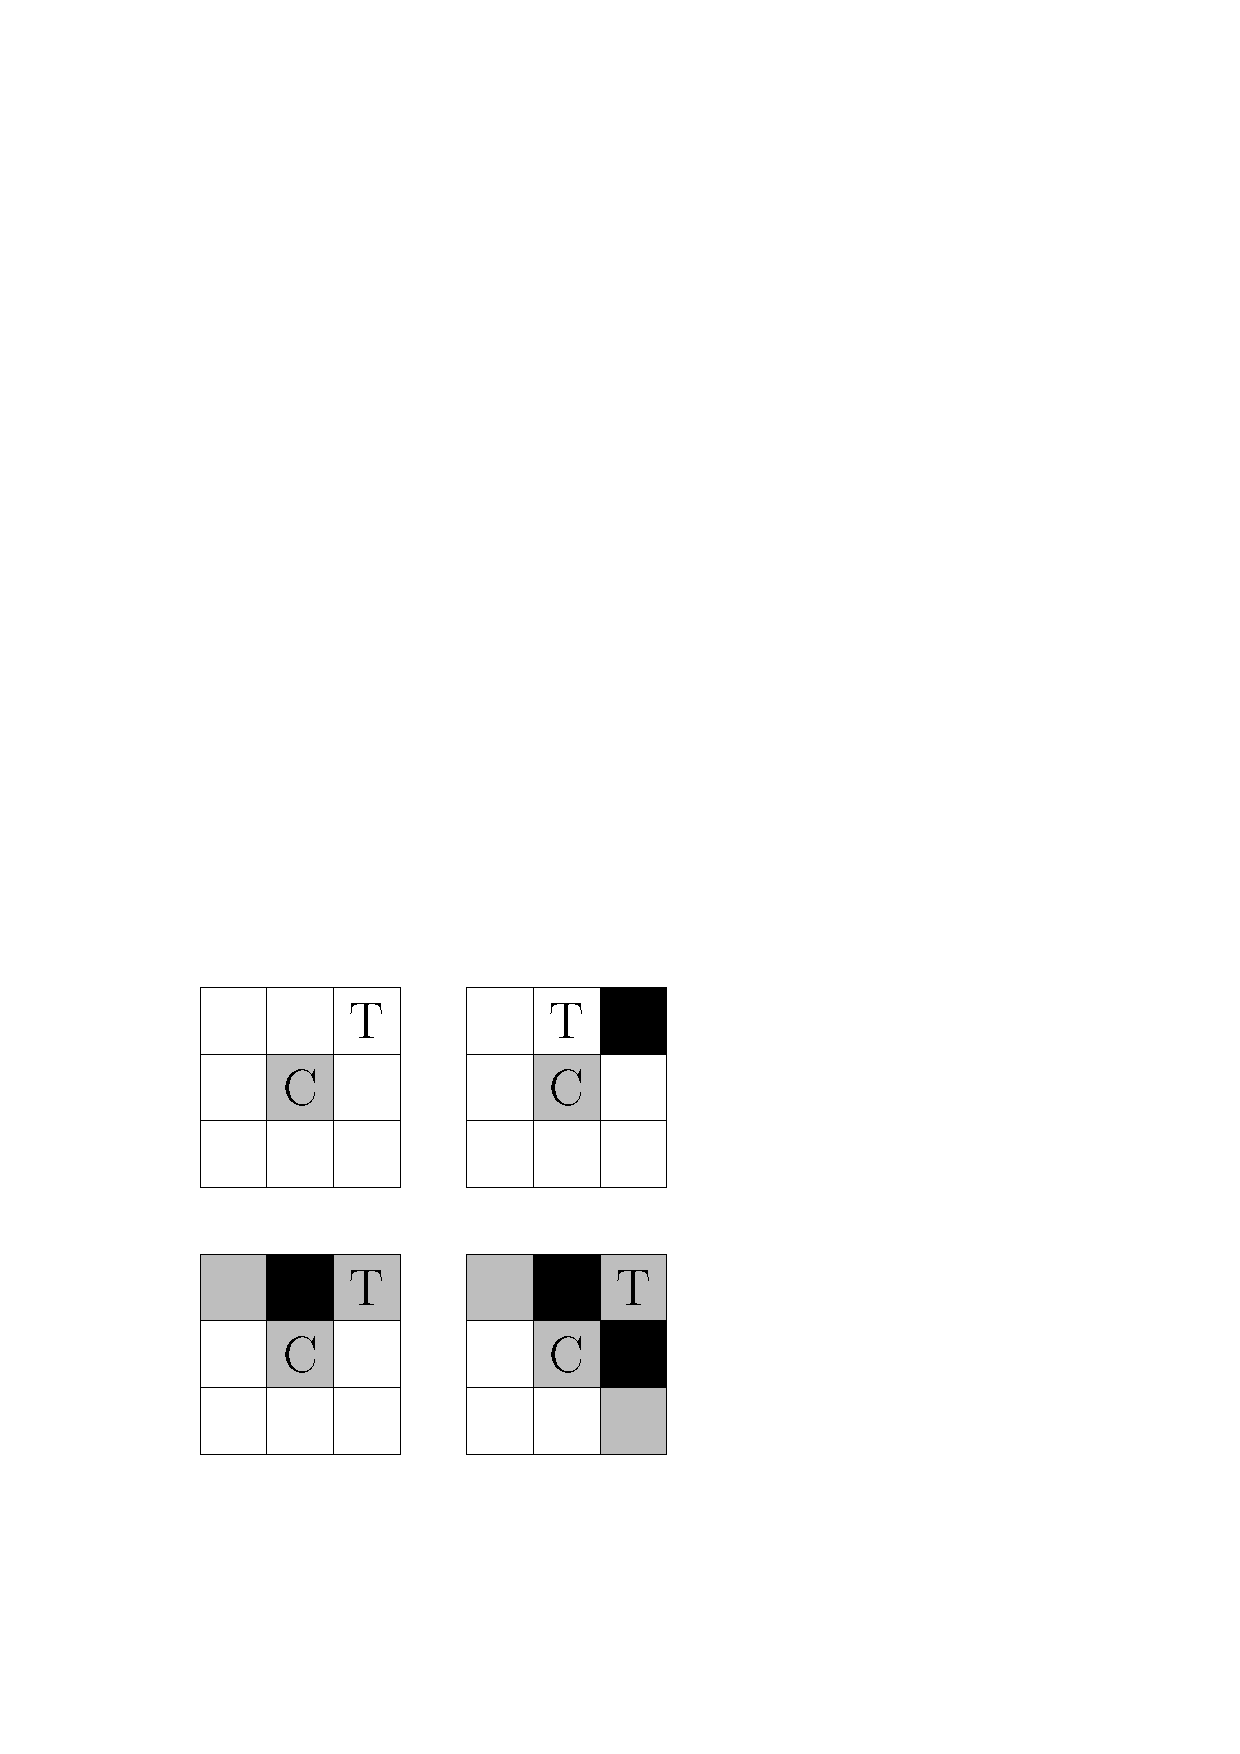
\includegraphics[width=0.30\textwidth]{../images/diagonal_moves.pdf}
\caption{Diagonal movement}
\label{fig:diag_move}
\end{wrapfigure}

Solid, static obstacles on the map will have their cells marked, such that path finding is disallowed using these cells to pass through. We will allow diagonal steps in our paths, for more smooth movement, this does however bring a restriction. A diagonally adjacent cell is only considered a neighbour of the current cell if both cells directly adjacent to the target cell and the current cell are not obstacles. 

In figure \ref{fig:diag_move}, we see a current cell $C$ and a target cell $T$ in various situations. The upper left shows the neutral situation, all cells other than $C$ are white, meaning that $C$ can reach all of these cells in one step. In the upper right, we see an obstruction in the upper right corner, marked as black. The obstruction cannot be moved to, but since it is not directly adjacent to $C$, it does not hinder $C$ from going to $T$ (or the other way around). In the lower left image we see a situation of a square that is directly adjacent to both $C$ and $T$, this one prevents $C$ from directly stepping to $T$, as marked grey. Lastly, we get the situation that both adjacent cells are an obstruction, for completeness.

\subsubsection{Non-solid Obstacles}
Vikings will walk slower in the dark, whereas zombies will slow down in the light. Next to this, any number of terrain hazards may be added to the game. When finding a path this has to be taken into account. These obstructions mean that our navigation graph has to be weighted. A good algorithm for dealing with weighted graphs would be A*, which we will expand further on to accommodate the solutions for other problems.

Since we are navigating on a grid over the environment, each cell has its own terrain properties. Since the cells are essentially the nodes in the graph for the path finding algorithm, the weight of edges is more related to the nodes than the actual edges. We define an edge's weight by the weight of the node it points towards, in our directed graph. 

Lastly, the way of path following we take may form some sort of obstacles to particular paths. Our problem here is that we want smooth movement without game characters just walking through each other. This means that other characters need to somehow be taken into account when calculating the most practical path. Additional weighting criteria can be put on the cells in our grid depending on the circumstances. In section \ref{sec:extra_weight} we explain how this extra weighting will be done to accommodate our chosen path following approach. Next to this, we currently also increase the weight of cells that are occupied at the time of path-finding, as these might be characters blocking off narrow pathways.

\subsubsection{A*}
The obvious first step to take when choosing a path finding algorithm is to check out if A* fits. In our case, sofar, yes it does. A* is a generalisation of Dijkstra's algorithm, which is essentially A* with $0$ as a heuristic. A* uses a distance heuristic to estimate how close cells are to the target cell. To find the optimal path, this heuristic must always return an underestimate. This algorithm makes use of the fact that we only need to know a path between one point, not from one point to all. Essentially, what A* does differently from Dijkstra is determining the order in which it evaluates nodes, in order to sooner reach its target. A* adds the heuristic score of a node to the path length to that node and uses that as base for sorting its evaluation queue, rather than just the path length. For as far as our game is developed, this algorithm gets the job done.

\subsubsection{Limited Knowledge}
For our game we will deal with a ``fog of war'' for a group or a limited viewing radius of individual units. This means that a path cannot simply be planned out completely with A*. One solution for this is to have A* recalculate from a new position after information has been gathered along the path, but this would be very slow. Instead, we are better off using an incremental variant of A*, called D*. D* uses data from prior calculations towards the same goal to more efficiently find an alternative path. We will be opting for a more simple and efficient version of D*, D*-Lite. D*-Lite is based on Lifelong Planning A*, thus giving it a different algorithmic structure from plain D*, but the same navigational strategy. Sadly, our game did not make it to the point of this mechanic becoming relevant.

\subsubsection{D*-Lite}
We ended up not implementing this algorithm since we did not reach the need for it yet, both in mechanics and scale. Because of this, the explanation given in this section will be brief and basic, unless suggested otherwise as feedback.

D*-Lite is a similar algorithm to A*, with the added advantage that it remembers old data it gathered when planning to a target point, such that replanning can be done more efficiently. A notable difference is that D*-lite essentially uses the strategy of A* in reverse, it computes from goal node to start node. The heuristic value hence indicates the estimate distance of a node to the original start node. The so called ``g-value'' refers to the computed distance between a cell and the goal node. Next to this, a value called the rhs-value is maintained, which is determined as the minimum over all its neighbours of the g-value of its neighbour plus the distance between the two of them.

When the situation changes and a cell is found to have a different weight than expected, recalculations are done. The changed node has its rhs-value recalculated. If the rhs-value does not match its old g-value, the node is locally inconsistent, the change influenced it. If it is inconsistent, it is added back into the queue for evaluation. When a node gets evaluated again, it can either trigger the simple re-evaluation of its predecessors (the neighbours in the direction of the goal), or the update and re-evaluation of them. When re-evaluation concludes, a new path can be found through back-pointers from wherever the character is in the evaluated grid.

\subsubsection{Distance Heuristics}
Our path finding algorithms, as well as some other things, require heuristics to estimate distances. In the case of path finding, these heuristics have to underestimate the actual distance for the purposes of comparing to partially found paths. The larger the lower bound the heuristic gives is, the faster our path finding will be. In the event that we decide to speed up the algorithms by finding non-optimal paths, the accuracy of the used heuristic will also impact the quality of the path. Each of the heuristics introduced here, except Manhattan on diagonals, gives a underestimate of the requested distance, not taking into account potential obstacles. 

Each heuristic is accompanied by a certain shape. The shape of a heuristic is a scalar polygon that shows what a returned distance $r$ from its calculation means for the different angles between the focal (center) point and the compared (border) point. The smaller the shape, the higher the lower bound it gives is. Shapes are typically more accurate if they conform to the individual moves the path finding algorithm can take, the directions in which one cell can lie relative to the previous cell in the path. 

In each heuristic formula, we will refer to the coordinates as $x_i$ and $y_i$ for $x$ and $y$ coordinates, respectively, where $i \in \{ 1, 2\}$.

\paragraph{Euclidean}
\label{sec:euclidean}
\begin{wrapfigure}{r}{0.30\textwidth}
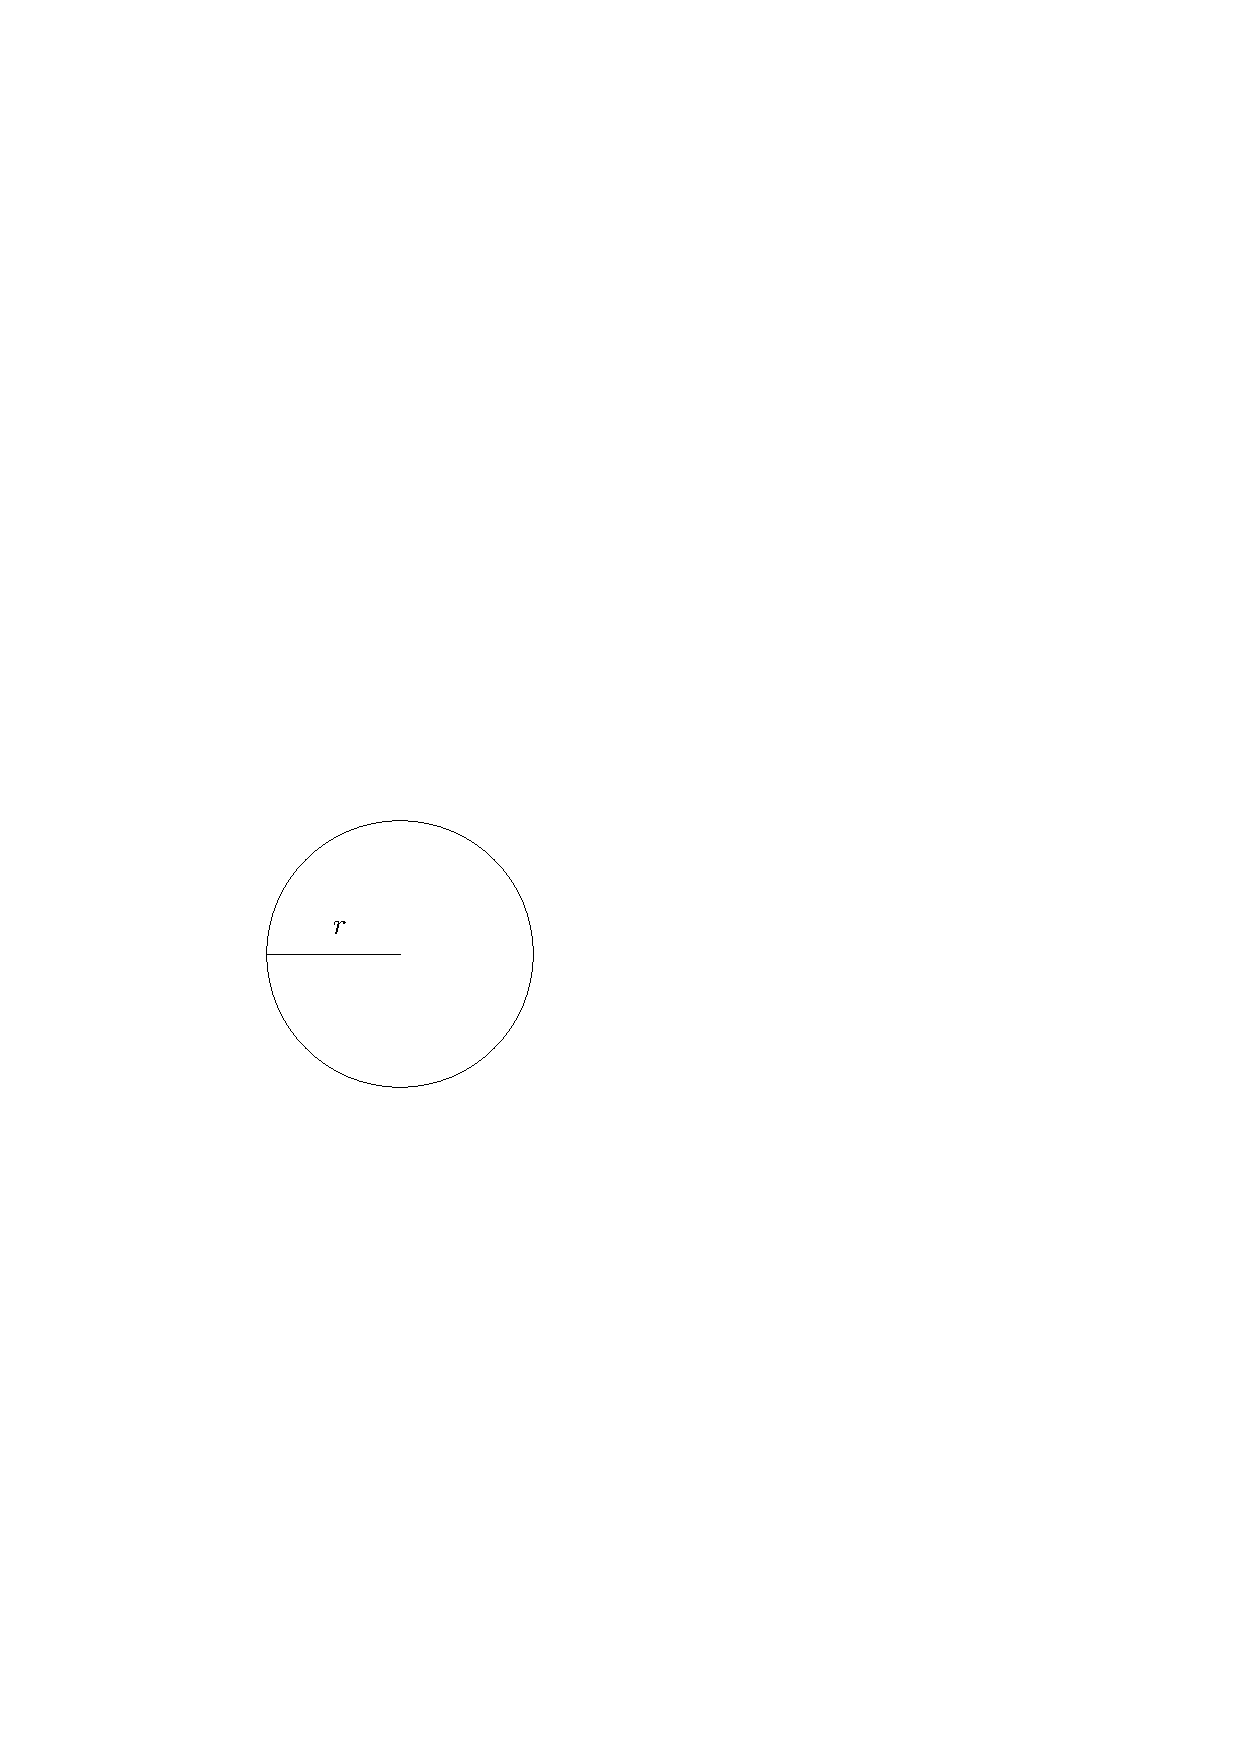
\includegraphics[width=0.30\textwidth]{../images/euclidean_unit.pdf}
\caption{Euclidean distance shape}
\end{wrapfigure}
Our first heuristic, and the one we have used in our system, is the Euclidean distance. Euclidean distance is given by $\sqrt{(x_1 - x_2)^2 + (y_1 - y_2)^2}$. We went for this heuristic, as it conforms with our ideals of movement, using any direction.

In retrospect, this was not the best decision, as the heuristic is meant for speeding up the algorithm, rather than steering towards desired resulting paths. The main downside of this heuristic is that we need to calculate a square root, which is a potential bottleneck for performance. Instead of using Math.sqrt, we may opt for a close approximation, in case performance becomes a problem. The following piece of code is used in Java to approximate the square root "rootOfValue" of the input "value":
\begin{lstlisting}
float sqrtApprox(float value) {
	float number = value;
	float xhalf = 0.5f*number;
	int i = Float.floatToIntBits(number);
	i = 0x5f3759df - (i>>1);
	number = Float.intBitsToFloat(i);
	number = number*(1.5f - xhalf*number*number);
	float rootOfValue = 1/number;
	return rootOfValue;
}
\end{lstlisting}

\paragraph{Manhattan}
\begin{wrapfigure}{r}{0.30\textwidth}
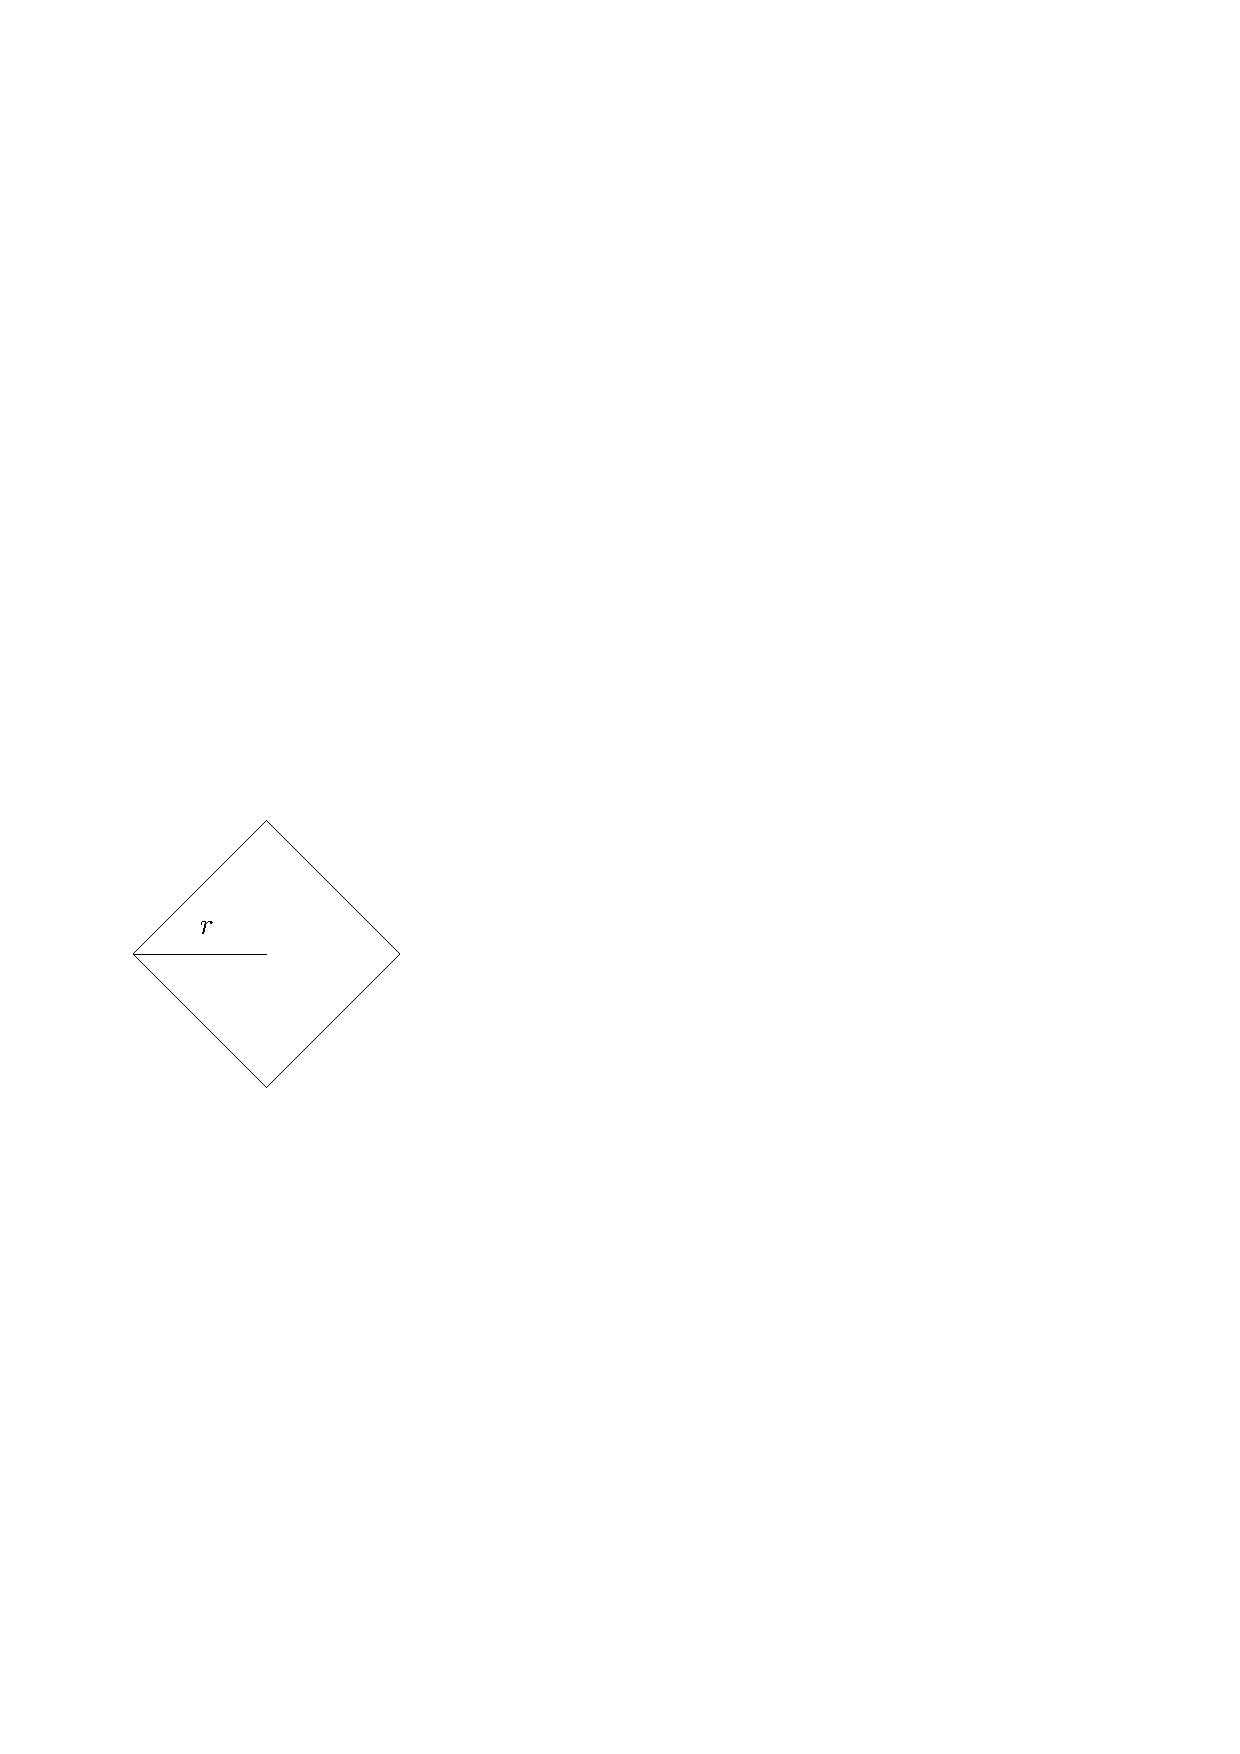
\includegraphics[width=0.30\textwidth]{../images/manhattan_unit.pdf}
\caption{Manhattan distance shape}
\end{wrapfigure}
The second heuristic we considered is the Manhattan distance. Manhattan distance is given by $\lvert x_1 - x_2 \rvert + \lvert y_1 - y_2 \rvert$. In the simulations we looked at, this heuristic typically had the fastest results. 

The problem that arose with this was that our path-finding also considers diagonal neighbours in the grid. Manhattan distance overestimates diagonal distances, since we count them as $\sqrt{2}$ rather than $2$. The reason we did not simply consider only using vertical and horizontal neighbours was that we wanted movement to be smooth-looking, so $8$ directions fits much more with our requirements than $4$.

\paragraph{Chebyshev}
\label{sec:chebyshev}
\begin{wrapfigure}{r}{0.30\textwidth}
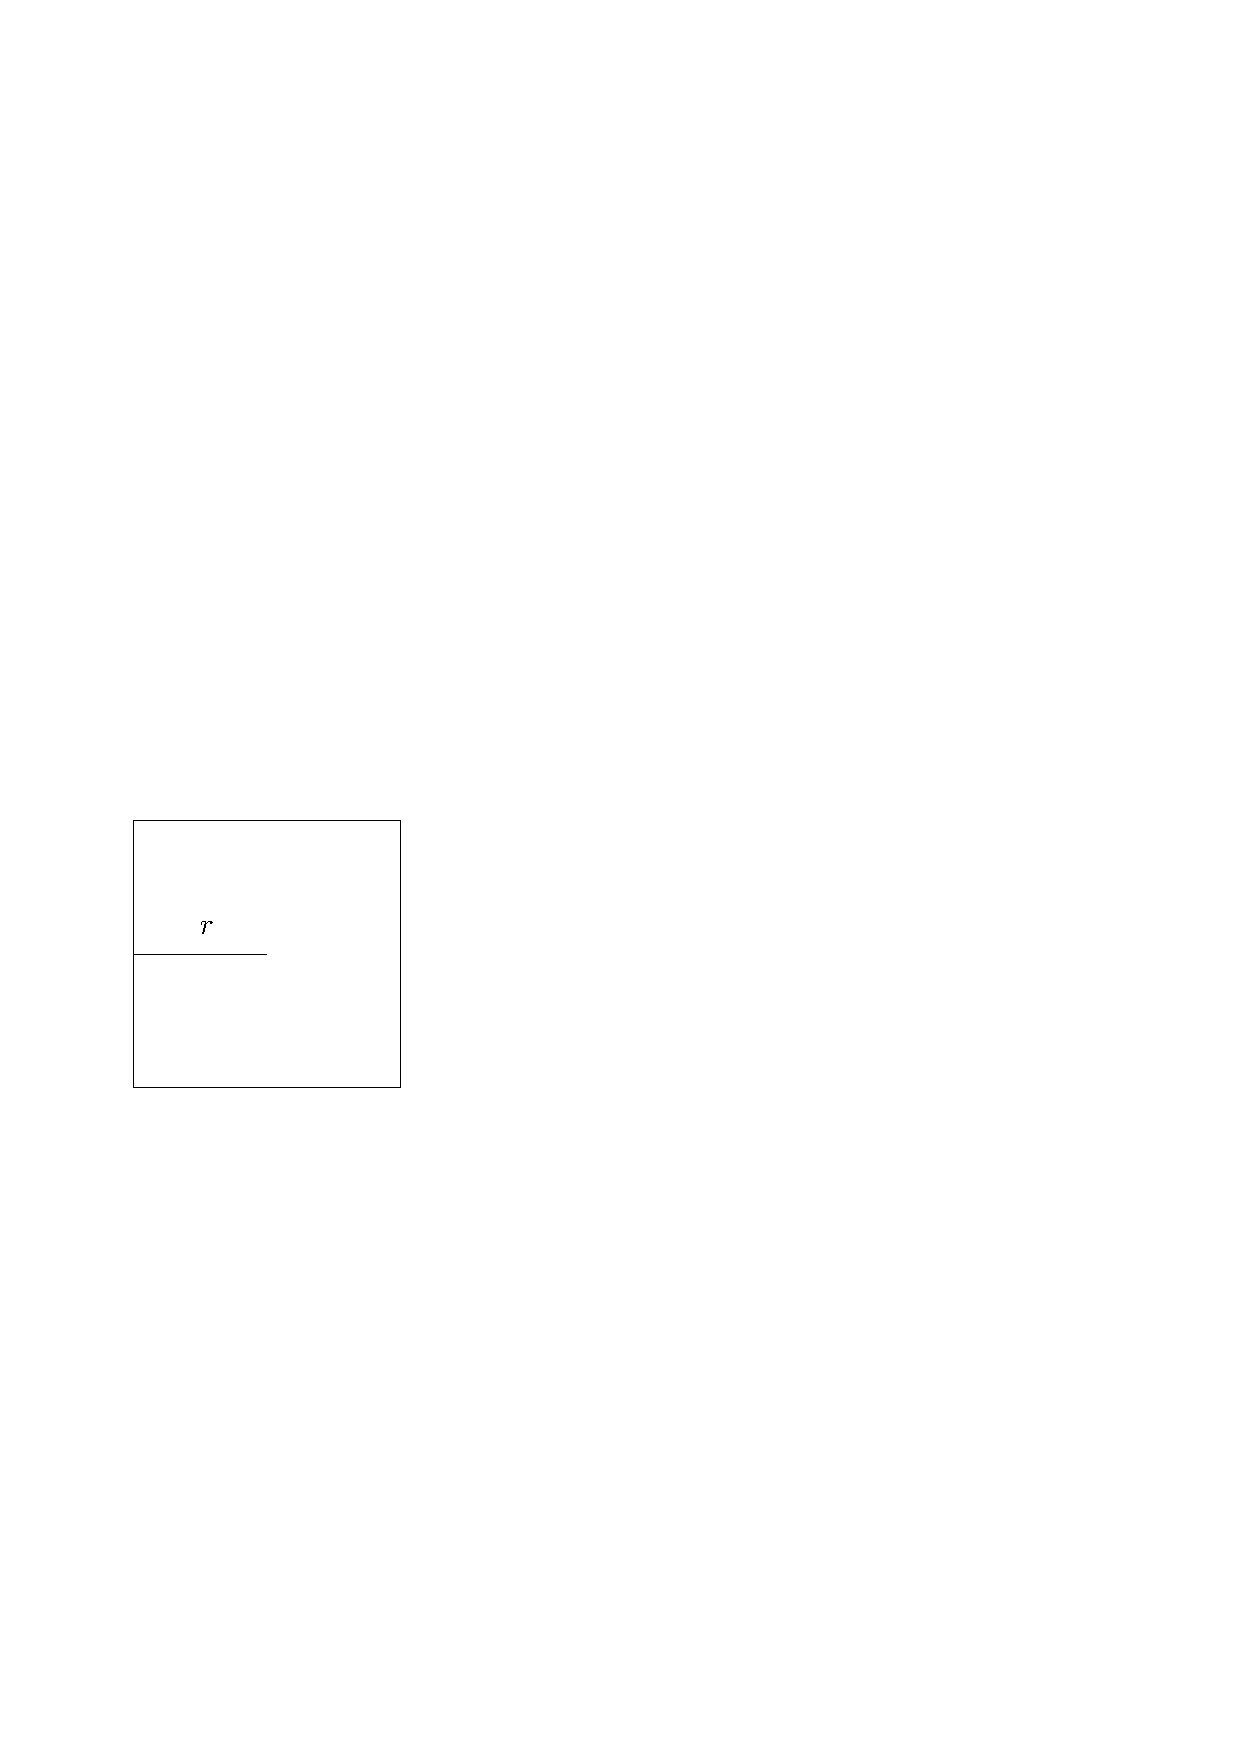
\includegraphics[width=0.30\textwidth]{../images/chebyshev_unit.pdf}
\caption{Chebyshev distance shape}
\end{wrapfigure}
To complete the triad of distance heuristics, we also considered Chebyshev distance as our third option. Chebyshev distance is given by $max(\lvert x_1 - x_2 \rvert, \lvert y_1 - y_2 \rvert)$. Like Manhattan distance, this heuristic worked fast and well in the simulations we looked at, though it was slightly below Manhattan in performance.

The main problem with this heuristic is that the diagonal movement, once again, is not taken into account. This time, we get that the heuristic sees diagonal movement as distance $1$ instead of $\sqrt{2}$ or $2$ for Manhattan. This means that the algorithm will typically go for a lot of horizontal or vertical steps first, as the distance for diagonal steps goes up a lot faster than the heuristic score goes down.

There is a benefit to this heuristic in the shape it forms. The square shape conforms to the shape of the grid, which means we can possibly apply it to other areas. We have applied this heuristic for a different purpose in section \ref{sec:solid_cells}.

\paragraph{Diagonal Manhattan}
\begin{wrapfigure}{r}{0.30\textwidth}
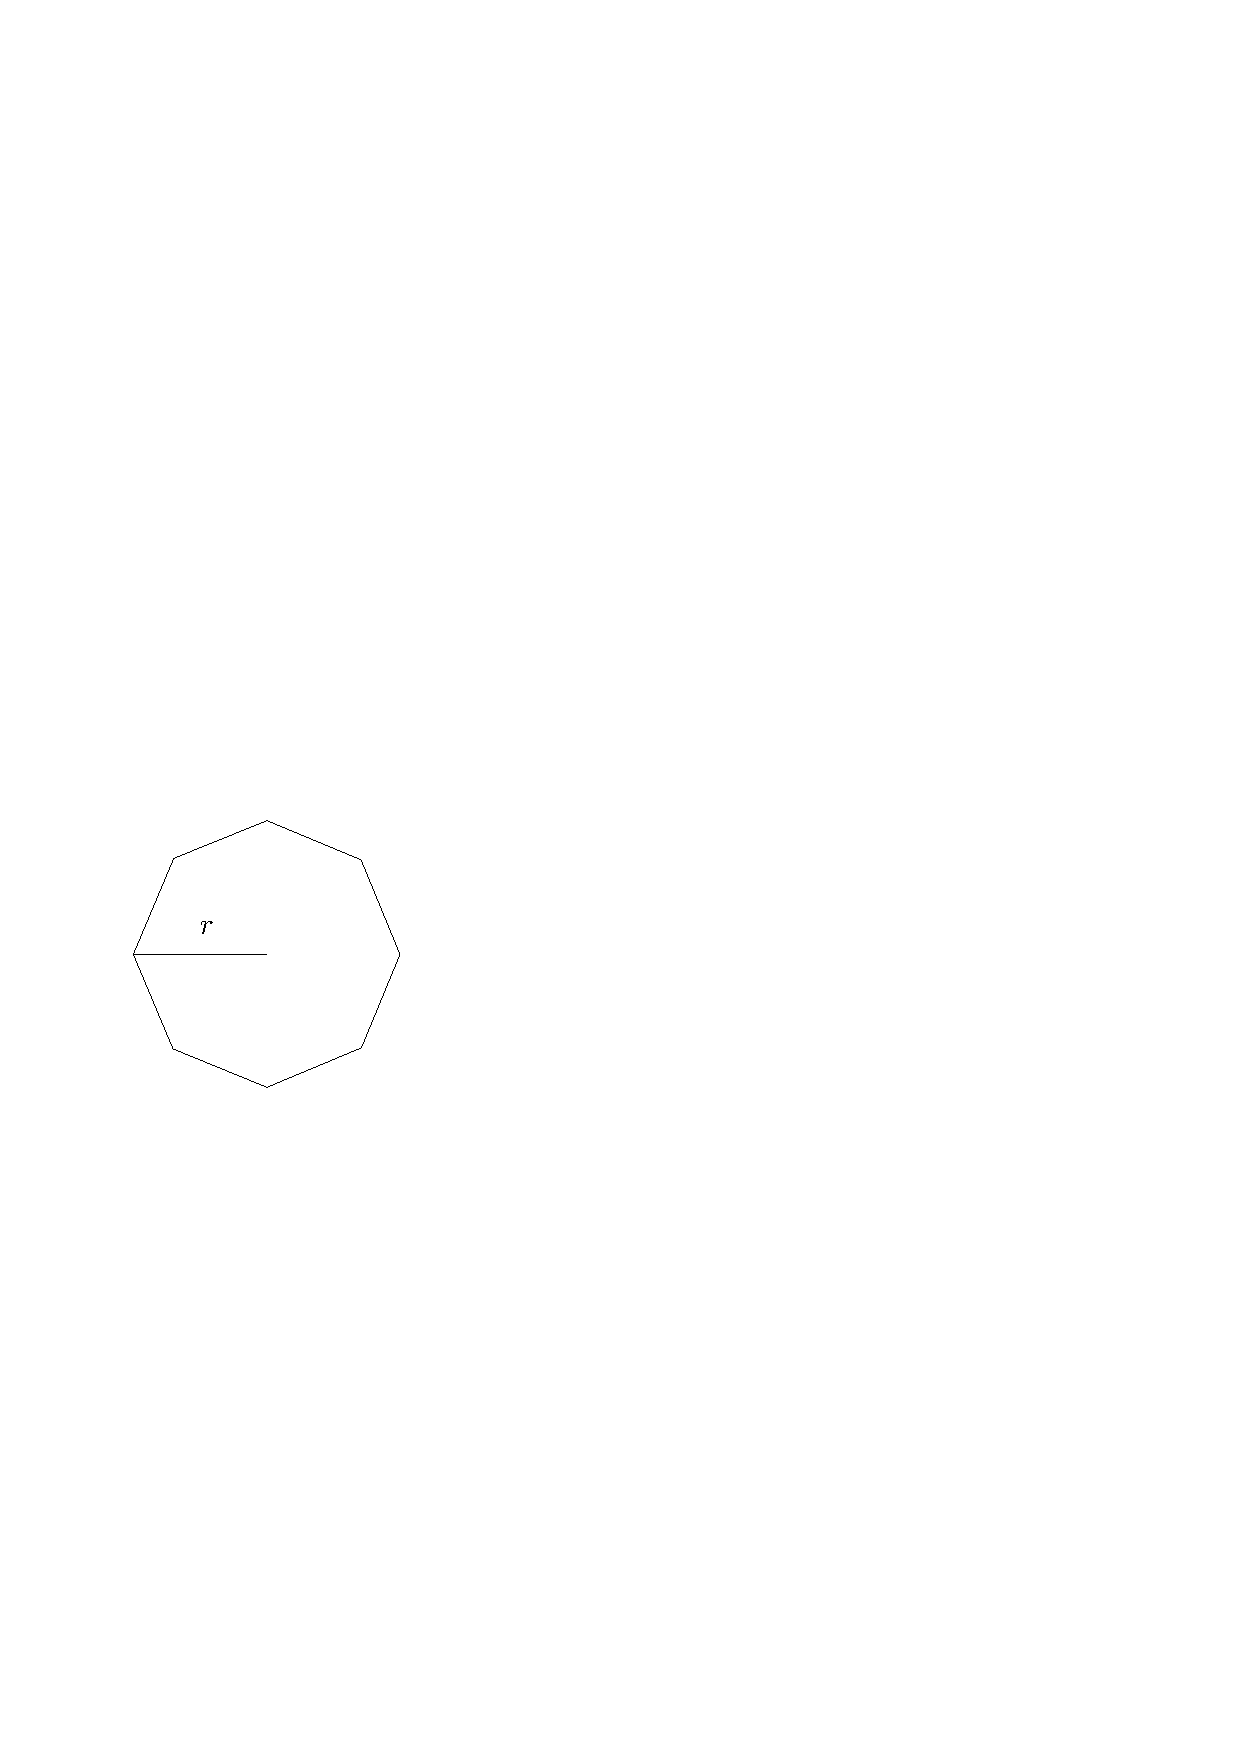
\includegraphics[width=0.30\textwidth]{../images/diagonal_manhattan_unit.pdf}
\caption{Diagonal Manhattan distance shape}
\end{wrapfigure}
Diagonal Manhattan distance is our own hybrid between between Manhattan and Chebyshev distance. The distance is given by $max(\lvert x_1 - x_2 \rvert, \lvert y_1 - y_2 \rvert) + min(\lvert x_1 - x_2 \rvert, \lvert y_1 - y_2 \rvert) * (\sqrt{2} - 1)$. What this formula does is add the diagonal distance, as per Euclidean calculation, to the remaining Manhattan distance in one straight line. In essence, we take Chebyshev distance, and multiply it by the Euclidean distance for a single diagonal move, excluding the remaining purely horizontal or vertical distance. The calculation comes from taking the whole Chebyshev distance, considered as a straight line, and add the distance that actually needs to be diagonal to the total, scaled by the difference in distance between two horizontally or vertically adjacent cells, and the distance between two diagonally adjacent cells.

This is, logically speaking, the best out of these heuristics for path finding purposes. The estimated distance is the exact distance the path would be if there were no obstacles along the way, when using horizontal, vertical and diagonal moves. We ended up not replacing Euclidean distance by this heuristic, as we did not yet require performance enhancement to path finding, given our progress. Additionally, this is only theoretical, we have not seen simulations with this heuristic and have not had the time to test it ourselves.

\subsubsection{Other performance enhancements}
We want our maps to be large and the number of zombies to be great, so paths to be calculated have to be long and plentiful. In order to do this, we need to make sure that our path finding is extra efficient. Due to the progress made in development, none of these techniques have been required or used. 

\paragraph{Heuristic Weighting}
We can use the fact that A* can be adjusted to make sub-optimal paths and apply it to D*-Lite, should we switch to that. The output of the heuristic function used to estimate distance to the goal can be multiplied by $1 + \epsilon$, Static Heuristic Weighting (SHW). This way, the evaluated points that are already close to the goal take priority over those still around the starting point. The value of $\epsilon$ can even be adjusted according to the current performance. We did not use this yet, as it was not deemed necessary in the current state of the game

\paragraph{Obstacle Approximation}


\paragraph{Typical Path Finding Speed-Up}
We have briefly looked into some conventional performance enhancements for A*. The most notable enhancement options we found are Dead End Detection (DED) and Minimal-Memory Abstraction (MMA). These ideas were scrapped due to time constraints, as they were looked into rather late. 

Dead End Detection does exactly what it sounds like. In order to prevent needlessly evaluating all the nodes in a dead end, we can use a few methods to skip them entirely. Given the right kind of maps and the need for performance enhancements, this is something to look into more in the future.

Minimal-Memory Abstraction looks at the structure of the map and isolates spaces in which can be more or less freely moved. Instead of running path finding on the huge graph that is the map grid, it runs on a graph made up of isolated spaces. The paths between spaces can be calculated without too much trouble. This would be a very powerful tool, if our characters had complete knowledge of the map. The fact that characters may not know everything of the map makes this approach give relatively unrealistic results, as well as requiring some mapping of grid exploration to abstract graph exploration.

\paragraph{Neighbour Pruning}
Neighbour pruning is a principle that essentially crops the graph your path finding works with. The two methods considered are called Rectangular Symmetry Reduction (RSR)and Jump Point Search (JPS), which are forms of Symmetry Breaking. These methods were considered as an emergency performance improvement, in case of heavy speed drops. The problem with using RSR or JPS is that it does not take into account edge weights, so avoidance of non-solid obstacles gets ignored. In the demonstrations we have seen, the pruning itself actually cost a lot of time in certain situations. The fact that we cannot easily predict when pruning actually helps, along with the added effort for having to implement it made us drop these ideas entirely.

Rectangular Symmetry Reduction works similar to abstraction from individual cells. The map is processed and decomposed into rectangular, symmetric areas. These areas can be used as points in path finding individually, while calculating how to traverse the rectangle itself is kept simple.

Jump Point Search uses looking ahead over straight lines to isolate which cells are actually relevant for finding a working path. This makes the space over which we have to calculate a path dramatically smaller. The resulting path is a sequence of jumps, which can be easily filled in to form a sequence of neighbours.

\paragraph{Flocking Only}
The most efficient way of improving an algorithm's performance is to not require using it. We considered the simple idea of having Flocking handle everything itself. Although flocking is a good tool on its own in many situations, it cannot find its way through more complex areas. Considering the setting of the game, we will likely have urban location with non-trivial navigation.

\paragraph{Minimal Updating}
If we still were to go for the usage of ``fog of war'', the question arises of when to re-evaluate a path and how frequently. This can be done at an absolute minimum by waiting until an occupied cell is the next cell in a path.
